% Options for packages loaded elsewhere
\PassOptionsToPackage{unicode}{hyperref}
\PassOptionsToPackage{hyphens}{url}
%
\documentclass[
  ignorenonframetext,
]{beamer}
\usepackage{pgfpages}
\setbeamertemplate{caption}[numbered]
\setbeamertemplate{caption label separator}{: }
\setbeamercolor{caption name}{fg=normal text.fg}
\beamertemplatenavigationsymbolsempty
% Prevent slide breaks in the middle of a paragraph
\widowpenalties 1 10000
\raggedbottom
\setbeamertemplate{part page}{
  \centering
  \begin{beamercolorbox}[sep=16pt,center]{part title}
    \usebeamerfont{part title}\insertpart\par
  \end{beamercolorbox}
}
\setbeamertemplate{section page}{
  \centering
  \begin{beamercolorbox}[sep=12pt,center]{part title}
    \usebeamerfont{section title}\insertsection\par
  \end{beamercolorbox}
}
\setbeamertemplate{subsection page}{
  \centering
  \begin{beamercolorbox}[sep=8pt,center]{part title}
    \usebeamerfont{subsection title}\insertsubsection\par
  \end{beamercolorbox}
}
\AtBeginPart{
  \frame{\partpage}
}
\AtBeginSection{
  \ifbibliography
  \else
    \frame{\sectionpage}
  \fi
}
\AtBeginSubsection{
  \frame{\subsectionpage}
}
\usepackage{amsmath,amssymb}
\usepackage{iftex}
\ifPDFTeX
  \usepackage[T1]{fontenc}
  \usepackage[utf8]{inputenc}
  \usepackage{textcomp} % provide euro and other symbols
\else % if luatex or xetex
  \usepackage{unicode-math} % this also loads fontspec
  \defaultfontfeatures{Scale=MatchLowercase}
  \defaultfontfeatures[\rmfamily]{Ligatures=TeX,Scale=1}
\fi
\usepackage{lmodern}
\usetheme[]{Madrid}
\ifPDFTeX\else
  % xetex/luatex font selection
\fi
% Use upquote if available, for straight quotes in verbatim environments
\IfFileExists{upquote.sty}{\usepackage{upquote}}{}
\IfFileExists{microtype.sty}{% use microtype if available
  \usepackage[]{microtype}
  \UseMicrotypeSet[protrusion]{basicmath} % disable protrusion for tt fonts
}{}
\makeatletter
\@ifundefined{KOMAClassName}{% if non-KOMA class
  \IfFileExists{parskip.sty}{%
    \usepackage{parskip}
  }{% else
    \setlength{\parindent}{0pt}
    \setlength{\parskip}{6pt plus 2pt minus 1pt}}
}{% if KOMA class
  \KOMAoptions{parskip=half}}
\makeatother
\usepackage{xcolor}
\newif\ifbibliography
\usepackage{graphicx}
\makeatletter
\def\maxwidth{\ifdim\Gin@nat@width>\linewidth\linewidth\else\Gin@nat@width\fi}
\def\maxheight{\ifdim\Gin@nat@height>\textheight\textheight\else\Gin@nat@height\fi}
\makeatother
% Scale images if necessary, so that they will not overflow the page
% margins by default, and it is still possible to overwrite the defaults
% using explicit options in \includegraphics[width, height, ...]{}
\setkeys{Gin}{width=\maxwidth,height=\maxheight,keepaspectratio}
% Set default figure placement to htbp
\makeatletter
\def\fps@figure{htbp}
\makeatother
\setlength{\emergencystretch}{3em} % prevent overfull lines
\providecommand{\tightlist}{%
  \setlength{\itemsep}{0pt}\setlength{\parskip}{0pt}}
\setcounter{secnumdepth}{-\maxdimen} % remove section numbering
\ifLuaTeX
  \usepackage{selnolig}  % disable illegal ligatures
\fi
\usepackage{bookmark}
\IfFileExists{xurl.sty}{\usepackage{xurl}}{} % add URL line breaks if available
\urlstyle{same}
\hypersetup{
  pdftitle={1 - Transmissores e modulações digitais},
  pdfauthor={TDI Course},
  hidelinks,
  pdfcreator={LaTeX via pandoc}}

\title{1 - Transmissores e modulações digitais}
\author{TDI Course}
\date{}

\usepackage{tikz}
\usetikzlibrary{shapes.geometric, positioning, arrows.meta, calc, backgrounds}

% Define a clean and pleasing color scheme
\definecolor{bitgreen}{RGB}{204, 255, 204}
\definecolor{discretedyellow}{RGB}{255, 255, 204}
\definecolor{rforange}{RGB}{255, 229, 204}
\definecolor{channelblue}{RGB}{204, 229, 255}

\begin{document}
\frame{\titlepage}

\section{Introdução à Transmissão Digital da Informação}\label{sec1}

\begin{frame}{Sistemas de Transmissão Digital da Informação}
Num sistema de comunicação digital a função do transmissor é converter
uma dada sequência de bits num trem de pulsos elétricos que, por sua
vez, poderar ser utilizado na modulação de uma portadora.


\includegraphics{figuras/Fig1.png}

%\begin{figure}
%        \centering
%        % O comando \resizebox ajusta o diagrama à largura exata do slide
%        \resizebox{\textwidth}{!}{%
%        \begin{tikzpicture}[
%            node distance=0.8cm and 0.6cm, % Espaçamento horizontal e vertical reduzidos
%            block/.style={rectangle, draw, thin, rounded corners=0.15cm, minimum width=2.4cm, minimum height=1.2cm, align=center, fill=white, text width=2.2cm, font=\scriptsize},
%            bit_block/.style={block, fill=bitgreen},
%            discrete_block/.style={block, fill=discretedyellow},
%            rf_small/.style={block, fill=rforange, minimum width=0.9cm, minimum height=0.8cm, text width=0.8cm},
%            channel_block/.style={ellipse, draw, thick, minimum width=3.2cm, minimum height=1.8cm, align=center, fill=channelblue, text width=2.8cm, font=\footnotesize\bfseries},
%            arrow/.style={-Latex, thick},
%            signal_label/.style={align=center, font=\scriptsize\bfseries}
%        ]
%
%        % ---------------------------------------------------------
%        % BLOCOS DO TRANSMISSOR (Tx)
%        % ---------------------------------------------------------
%        \node[bit_block] (Tx_A1) {Fonte de inf.\\binária (bits)};
%        \node[bit_block, right=of Tx_A1] (Tx_A2) {Codificador\\de canal};
%        \node[discrete_block, right=of Tx_A2] (Tx_A3) {Modulador\\Digital (map)};
%        \node[inner sep=2pt, right=of Tx_A3, xshift=-0.2cm] (Tx_A4) {\Large$\uparrow$};
%        \node[discrete_block, right=of Tx_A4] (Tx_A5) {Filtro\\Formatador};
%        \node[rf_small, right=0.6cm of Tx_A5, yshift=0.5cm] (Tx_DAC_I) {DAC};
%        \node[rf_small, below=0.1cm of Tx_DAC_I] (Tx_DAC_Q) {DAC};
%
%        % ---------------------------------------------------------
%        % BLOCOS DO RECEPTOR (Rx)
%        % ---------------------------------------------------------
%        \node[bit_block] (Rx_B1) [below=2.8cm of Tx_A1] {Informação\\recuperada};
%        \node[bit_block, right=of Rx_B1] (Rx_B2) {Decodificador\\de canal};
%        \node[discrete_block, right=of Rx_B2] (Rx_B3) {Demodulador\\Digital (demap)};
%        \node[inner sep=2pt, right=of Rx_B3, xshift=-0.2cm] (Rx_B4) {\Large$\downarrow$};
%        \node[discrete_block, right=of Rx_B4] (Rx_B5) {Filtro\\Casado};
%        \node[rf_small, right=0.6cm of Rx_B5, yshift=0.5cm] (Rx_ADC_I) {ADC};
%        \node[rf_small, below=0.1cm of Rx_ADC_I] (Rx_ADC_Q) {ADC};
%
%        % ---------------------------------------------------------
%        % CANAL DE COMUNICAÇÕES
%        % ---------------------------------------------------------
%        \node[channel_block] (Channel) at ($(Tx_DAC_I.east)!0.5!(Rx_ADC_I.east) + (4.0cm, 0)$) {Canal de\\comunicações};
%
%        % Títulos Principais
%        \node[font=\normalsize\bfseries] (Transmitter_Label) [above=0.2cm of Tx_A1.north west, anchor=south west] {Transmissor};
%        \node[font=\normalsize\bfseries] (Receiver_Label) [above=0.2cm of Rx_B1.north west, anchor=south west] {Receptor};
%
%        % Conexões Tx
%        \draw[arrow] (Tx_A1) -- (Tx_A2);
%        \draw[arrow] (Tx_A2) -- (Tx_A3);
%        \draw[arrow] (Tx_A3) -- (Tx_A4);
%        \draw[arrow] (Tx_A4) -- (Tx_A5);
%        \draw[arrow] (Tx_A5.east) |- (Tx_DAC_I.west) node[midway, above, font=\tiny, xshift=0.1cm] {I};
%        \draw[arrow] (Tx_A5.east) |- (Tx_DAC_Q.west) node[midway, below, font=\tiny, xshift=0.1cm] {Q};
%
%        % ---------------------------------------------------------
%        % FRONT-END DE RF - TRANSMISSOR
%        % ---------------------------------------------------------
%        \begin{scope}
%            \node (Tx_Mix_I) at ($(Tx_DAC_I.east) + (1.2cm, 0)$) [circle, draw, minimum size=0.4cm, inner sep=0, font=\tiny] {X};
%            \node (Tx_Mix_Q) at ($(Tx_DAC_Q.east) + (1.2cm, 0)$) [circle, draw, minimum size=0.4cm, inner sep=0, font=\tiny] {X};
%            \node (Tx_LO) at ($(Tx_Mix_I.south)!0.5!(Tx_Mix_Q.north)$) [circle, draw, minimum size=0.4cm, inner sep=0, font=\tiny, label={right:\tiny$\sim$}] {};
%            \node (Tx_Comb) at ($(Tx_Mix_I.east) + (0.8cm, 0)$) [circle, draw, minimum size=0.4cm, inner sep=0, font=\tiny] {+};
%            \node[draw, rectangle, rounded corners=0.05cm, inner sep=1pt, font=\tiny, fill=white] (Pi2_Box) at ($(Tx_LO) + (0cm, 0.4cm)$) {$\pi/2$};
%            
%            \draw[arrow] (Tx_DAC_I) -- (Tx_Mix_I);
%            \draw[arrow] (Tx_DAC_Q) -- (Tx_Mix_Q);
%            \draw[->] (Tx_LO) -- (Pi2_Box);
%            \draw[->] (Pi2_Box) -- (Tx_Mix_I);
%            \draw[->] (Tx_LO) -- (Tx_Mix_Q);
%            \draw[->] (Tx_Mix_I) -| (Tx_Comb.north);
%            \draw[->] (Tx_Mix_Q) -| (Tx_Comb.south);
%            \draw[arrow] (Tx_Comb) -- (Channel.west);
%        \end{scope}
%
%        % ---------------------------------------------------------
%        % FRONT-END DE RF - RECEPTOR
%        % ---------------------------------------------------------
%        \begin{scope}
%            \node (Rx_Split) at ($(Channel.west) - (1.0cm, 0)$) [circle, draw, minimum size=0.4cm, inner sep=0, font=\tiny] {};
%            \node (Rx_Mix_I) at ($(Rx_Split.west) - (1.0cm, 0.5cm)$) [circle, draw, minimum size=0.4cm, inner sep=0, font=\tiny] {X};
%            \node (Rx_Mix_Q) at ($(Rx_Split.west) - (1.0cm, -0.5cm)$) [circle, draw, minimum size=0.4cm, inner sep=0, font=\tiny] {X};
%            \node (Rx_FPB_I) at ($(Rx_Mix_I.west) - (0.8cm, 0)$) [rectangle, draw, thin, minimum width=0.8cm, minimum height=0.6cm, inner sep=1pt, font=\tiny] {F.P.B};
%            \node (Rx_FPB_Q) at ($(Rx_Mix_Q.west) - (0.8cm, 0)$) [rectangle, draw, thin, minimum width=0.8cm, minimum height=0.6cm, inner sep=1pt, font=\tiny] {F.P.B};
%            \node (Rx_LO) at ($(Rx_Mix_I.south)!0.5!(Rx_Mix_Q.north)$) [circle, draw, minimum size=0.4cm, inner sep=0, font=\tiny, label={right:\tiny$\sim$}] {};
%            \node[draw, rectangle, rounded corners=0.05cm, inner sep=1pt, font=\tiny, fill=white] (Rx_Pi2_Box) at ($(Rx_LO) + (0cm, 0.4cm)$) {$\pi/2$};
%
%            \draw[arrow] (Channel.west) -- (Rx_Split);
%            \draw[->] (Rx_Split) -- ++(-0.2cm, 0) |- (Rx_Mix_I.east);
%            \draw[->] (Rx_Split) -- ++(-0.2cm, 0) |- (Rx_Mix_Q.east);
%            \draw[->] (Rx_LO) -- (Rx_Pi2_Box);
%            \draw[->] (Rx_Pi2_Box) -- (Rx_Mix_I);
%            \draw[->] (Rx_LO) -- (Rx_Mix_Q);
%            \draw[arrow] (Rx_Mix_I.west) -- (Rx_FPB_I.east);
%            \draw[arrow] (Rx_Mix_Q.west) -- (Rx_FPB_Q.east);
%            \draw[arrow] (Rx_FPB_I.west) -- (Rx_ADC_I.east);
%            \draw[arrow] (Rx_FPB_Q.west) -- (Rx_ADC_Q.east);
%        \end{scope}
%
%        % Conexões Rx
%        \draw[arrow] (Rx_ADC_I.west) |- ($(Rx_B5.east) + (0, 0.15cm)$) node[midway, above, font=\tiny, xshift=0.1cm] {I};
%        \draw[arrow] (Rx_ADC_Q.west) |- ($(Rx_B5.east) + (0, -0.15cm)$) node[midway, below, font=\tiny, xshift=0.1cm] {Q};
%        \draw[arrow] (Rx_B5) -- (Rx_B4);
%        \draw[arrow] (Rx_B4) -- (Rx_B3);
%        \draw[arrow] (Rx_B3) -- (Rx_B2);
%        \draw[arrow] (Rx_B2) -- (Rx_B1);
%
%        % ---------------------------------------------------------
%        % AGRUPAMENTOS VISUAIS DE PROCESSAMENTO
%        % ---------------------------------------------------------
%        \begin{scope}[on background layer]
%            \node[draw, dashed, fill=bitgreen!15, inner sep=0.2cm, fit=(Tx_A1) (Tx_A2) (Rx_B1) (Rx_B2), label={[above left, font=\footnotesize\bfseries, yshift=-0.1cm]:Bits}] {};
%            \node[draw, dashed, fill=discretedyellow!15, inner sep=0.2cm, fit=(Tx_A3) (Tx_A5) (Rx_B3) (Rx_B5), label={[above left, font=\footnotesize\bfseries, yshift=-0.1cm]:Sinais Discretos}] {};
%            \node[draw, dashed, fill=rforange!15, inner sep=0.2cm, fit=(Tx_DAC_I) (Tx_Comb) (Rx_ADC_Q) (Rx_FPB_Q), label={[above left, font=\footnotesize\bfseries, yshift=-0.1cm]:RF / Analógico}] {};
%        \end{scope}
%
%        \end{tikzpicture}%
%        }
%    \end{figure}

\end{frame}

\begin{frame}{Representações para a onda portadora}

Uma onda portadora contínua \(c(t)\) pode ser representada por

\begin{equation} c(t) = A \cos \left(2\pi f_c t + \theta\right) \end{equation}

em que \(t\) é o tempo em segundos, \(f_{c}\) em hertz é a frequência de
oscilação, \(A\) a amplitude e \(\theta\) a fase da onda portadora.

Podemos também escrever de forma alternativa:
\[ \begin{aligned}c(t) &= A \cos \left(2\pi f_c t + \theta\right)\\ &= \operatorname{Re}\left[A e^{j \theta} e^{j2\pi f_c t}\right] \end{aligned} \]
\end{frame}

\begin{frame}{Modulações digitais lineares}
\phantomsection\label{modulauxe7uxf5es-digitais-lineares}
Uma modulação digital é uma função \(F\) que mapeia bits ou conjuntos de
bits a símbolos (fasores) no plano complexo

\[ F: \{0, 1\}^k\rightarrow \{A_m,\theta_m\}_{m=1}^M\]

em que sequências de \(k\) bits são mapeadas num conjunto de \(M\)
símbolos (\(M=2^k\)).

Ex.1: \(\{0, 1\}\rightarrow \{(0, 0), (A, 0)\}\) (modulação OOK)

Ex.2: \(\{0, 1\}\rightarrow \{(A, 0), (A, \pi )\}\) (modulação BPSK)

Ex.3:
\(\{(0, 0),(0, 1),(1, 0),(1, 1)\}\rightarrow \{(0, 0), (A/3, 0), (2A/3, 0), (A, 0)\}\)
(modulação 4-PAM ou 4-ASK)

Ex.4:
\(\{(0, 0),(0, 1),(1, 0),(1, 1)\}\rightarrow \{(A, \pi/4), (A, 3\pi/4), (A, 5\pi/4), (A, 7\pi/4)\}\)
(modulação QPSK)
\end{frame}

\begin{frame}{Diagramas de constelação}
\phantomsection\label{diagramas-de-constelauxe7uxe3o}
\end{frame}

\begin{frame}{Parâmetros importantes das modulações digitais lineares}
\phantomsection\label{paruxe2metros-importantes-das-modulauxe7uxf5es-digitais-lineares}
Cardinalidade e número de bits por símbolo

A cardinalidade de uma modulação digital é definida como o número de
símbolos que compõem a sua constelação, geralmente indicada pela letra
\(M\). De modo a facilitar o mapeamento entre sequências binárias e
símbolos das constelações, \(M\) geralmente é uma potência inteira de 2,
ou seja, \(M=2^b\) onde \(b\) é o número de bits por símbolo
(bits/símbolo) da modulação. Quanto maior o valor de b, mais informação
pode ser carregada por cada símbolo transmitido. Entretanto, quanto
maior o valor de \(M\), maior a suscetibilidade dos sinais transmitidos
ao ruído e demais distorções que podem ser infligidas pelo canal de
comunicações.
\end{frame}

\begin{frame}{Energia média dos símbolos da constelação (\(E_s\))}
\phantomsection\label{energia-muxe9dia-dos-suxedmbolos-da-constelauxe7uxe3o-e_s}
Considere \(X\) uma variável aleatória discreta que representa a fonte
de símbolos do transmissor. Em cada instante de sinalização, o
transmissor envia para o canal um dos símbolos da constelação definida
por
\(\mathcal{X} = \left\lbrace s_0, s_1, \dots, s_{M-1}\right\rbrace\),
com probabilidade \(P(s_n),\;n = 0,1,\dots,M-1\), de modo que
\(\sum_{n=0}^{M-1}P(s_n)=1\). A energia média \(E_s\) dos símbolos
enviados pelo transmissor será dada pelo valor esperado:

\[\begin{aligned} E_s &= E\left[X^2\right] \\ &= \sum_{n=0}^{M-1}|s_n|^2P(s_n) \end{aligned} \]

Se cada um dos \(M\) símbolos ocorre com a mesma probabilidade, diz-se
que a fonte gera símbolos equiprováveis, de modo que
\(P(s_n)=\frac{1}{M}\). Neste caso, temos

\[ \begin{aligned} E_s &=\sum_{n=0}^{M-1}|s_n|^2\frac{1}{M} \\ &=  \frac{1}{M}\sum_{n=0}^{M-1}|s_n|^2\end{aligned} \]

Exemplos:

\begin{enumerate}
\tightlist
\item
  Considere a constelação 4-PAM definida por
  \(\mathcal{X} = \left\lbrace -3, -1, 1, 3\right\rbrace\). Considerando
  que os símbolos são gerados de maneira equiprovável, temos que:
\end{enumerate}

\[ \begin{aligned} E_s &=\sum_{n=0}^{M-1}|s_n|^2P(s_n) \\ &=  \frac{1}{4}\left[|-3|^2+|-1|^2+|1|^2+|3|^2\right] \\ &=  \frac{20}{4} = 5\end{aligned} \]

\begin{enumerate}
\setcounter{enumi}{1}
\tightlist
\item
  Considere a constelação 4-QAM definida por
  \(\mathcal{X} = \left\lbrace -1-j, -1+j, 1+j, 1-j\right\rbrace\).
  Considerando que os símbolos são gerados de maneira equiprovável,
  temos que:
\end{enumerate}

\[ \begin{aligned} E_s &=\sum_{n=0}^{M-1}|s_n|^2P(s_n) \\ &=  \frac{1}{4}\left[|-1-j|^2+|-1+j|^2+|1+j|^2+|1+j|^2\right] \\ &=  \frac{8}{4} = 2\end{aligned} \]

Logo, ao compararmos as modulações 4-PAM e 4-QAM dadas pelas
constelações descritas, nota-se que ao utilizar a constelação 4-PAM o
transmissor gastará, em média, \(2,5\times\) mais energia por símbolo
transmitido no canal do que gastaria utilizando a modulação 4-QAM.

Em diversas situações deseja-se comparar o desempenho entre diferentes
formatos de modulação num sistema de comunicações. Neste caso, comparar
constelações que possuem valores distintos de energia média por símbolo
pode causar inconsistências. Busca-se, então, normalizar a energia média
por símbolo das constelações, ou seja, fazer com que \(E_s = 1\), de
modo a garantir uma comparação justa. Desse modo assume-se que,
independentemente da modulação utilizada, o transmissor envia sempre a
mesma energia média por símbolo transmitido ao canal. A normalização é
feita dividindo-se os símbolos em \(\mathcal{X}\) por \(\sqrt{E_s}\).
Para verificar essa afirmação, podemos assumir que um fator
\(\alpha\in \mathbb{R}\) é utilizado para ampliar (\(\alpha>1\)) ou
reduzir (\(0<\alpha<1\)) as dimensões da constelação, de modo que
\(\mathcal{X} = \left\lbrace \alpha s_0,  \alpha s_1, \dots, \alpha s_{M-1}\right\rbrace\)
é a constelação resultante. Seja \(E_s^{(\alpha)}\) a nova energia média
por símbolo da constelação, temos que

\[\begin{aligned} E_s^{(\alpha)} &= \sum_{n=0}^{M-1}|\alpha s_n|^2P(s_n) \\ &= \alpha^2\sum_{n=0}^{M-1}|s_n|^2P(s_n) \\ &= \alpha^2 E_s\end{aligned} \]

Logo, se \(\alpha = \frac{1}{\sqrt{E_s}}\), então \(E_s^{(\alpha)}=1\).
\end{frame}

\begin{frame}{Distância euclidiana mínima entre símbolos (\(d_{min}\))}
\phantomsection\label{distuxe2ncia-euclidiana-muxednima-entre-suxedmbolos-d_min}
Para uma dada constelação
\(\mathcal{X} = \left\lbrace s_0, s_1, \dots, s_{M-1}\right\rbrace\), a
distância euclidiana mínima entre dois símbolos será dada por

\[d_{min} = \min_{i,k} |s_i-s_k| = \min_{i,k} \sqrt{(s_i-s_k)^2} \].

com \(i, k \in \left\lbrace 0, 1, \dots, M-1\right\rbrace\) e
\(i\neq k\).

Exemplos:

\begin{enumerate}
\item
  Considere a constelação 4-PAM normalizada definida por
  \(\mathcal{X} = \left\lbrace \frac{-3}{\sqrt{5}}, \frac{-1}{\sqrt{5}}, \frac{1}{\sqrt{5}}, \frac{3}{\sqrt{5}}\right\rbrace\),
  temos que \(d_{min}=\frac{2}{\sqrt{5}}\approx 0.894\).
\item
  Considere a constelação 4-QAM normalizada definida por
  \(\mathcal{X} = \left\lbrace \frac{-1-j}{\sqrt{2}}, \frac{-1+j}{\sqrt{2}}, \frac{1+j}{\sqrt{2}}, \frac{1-j}{\sqrt{2}}\right\rbrace\),
  temos que \(d_{min}=\frac{2}{\sqrt{2}}\approx 1.414\).
\end{enumerate}
\end{frame}


\begin{frame}{Intervalo de sinalização e taxa de símbolos}
\phantomsection\label{intervalo-de-sinalizauxe7uxe3o-e-taxa-de-suxedmbolos}
Num sistema de comunicações digitais, o transmissor envia bits pelo
canal de comunicações ao receptor em intervalos de tempo
pré-estabelecidos denominados \textbf{intervalo de sinalização}
(\(T_s\)). Diz-se que o transmissor ``faz uso do canal'' cada vez que
envia um símbolo de um esquema de modulação representando uma sequência
de bits. A taxa (ou frequência) em que símbolos são enviados pelo canal
para enviar símbolos é chamada de taxa (ou frequência) de sinalização
(\(R_s\)), ou taxa de símbolos, sendo medida em
\href{https://en.wikipedia.org/wiki/Baud}{baud}. A relação entre \(R_s\)
e \(T_s\) é dada por \(R_s=1/T_s\).

Quanto maior a taxa de símbolos, maior será a banda de espectro
necessária para a operação do sistema. Para recuperar corretamente a
sequência de símbolos transmitida, faz-se necessário que o transmissor e
receptor estejam \textbf{sincronizados}, ou seja, o receptor deve
conhecer exatamente os intervalos de sinalização utilizados pelo
transmissor para o envio da informação.

A quantidade de bits enviada em cada intervalo de sinalização
multiplicada por \(R_s\) corresponde à taxa de transmissão de bits do
sistema (\(R_b\)). Assumindo que cada símbolo de uma modulação digital
representa uma sequência de \(b\) bits, temos que:

\[R_b = kR_s \]

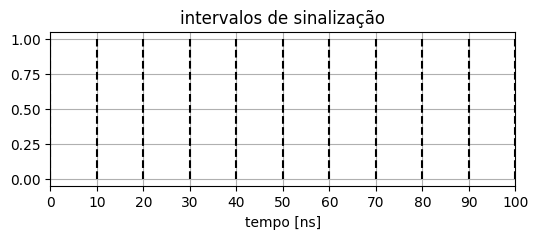
\includegraphics{figuras/nb0_out_0.png}
\end{frame}

\begin{frame}{Teorema da amostragem}
\phantomsection\label{teorema-da-amostragem}
O teorema de amostragem de \emph{Nyquist-Shannon} é um dos resultados
mais importantes utilizados em processamento digital de sinais, servindo
como uma ponte fundamental entre sinais de tempo contínuo e sinais de
tempo discreto. O teorema estabelece uma \textbf{condição suficiente}
para uma taxa de amostragem que permite que uma sequência discreta de
amostras capture toda a informação de um sinal contínuo no tempo e de
largura de banda finita.

Considerre \(x(t)\) um sinal limitado em banda, i.e.~o espectro de
frequências de \(X(f)=\mathcal{F}\{x(t)\}\) está contido no intervalo
\(-B\leq f \leq B\), ou seja

\[ X(f) = \int_{-\infty}^{\infty} x(t)e^{j2\pi f t} dt = 0 \text{, se } f < -B \text{ ou } f > B\]

Suponha que obtenhamos um sinal discreto no tempo \(x[k]\) a partir de
um conjunto de amostras equiespaçadas de \(x(t)\), ou seja
\(x[k]=x(kT_a)\), em que \(T_a = \frac{1}{f_a}\) é o período de
amostragem e \(f_a\) a frequência de amostragem.

Se \(f_a\geq 2B\), \(x(t)\) pode ser perfeitamente reconstruído a partir
de suas amostras \(x[k]\) fazendo

\[
x(t)=\sum_{n=-\infty}^{\infty} x(k T_a) \operatorname{sinc}\left(\frac{t-kT_a}{T_a}\right).
\]
\end{frame}
\begin{frame}{Exemplo 1: função sinc(t)}
\phantomsection\label{exemplo-1-funuxe7uxe3o-sinct}
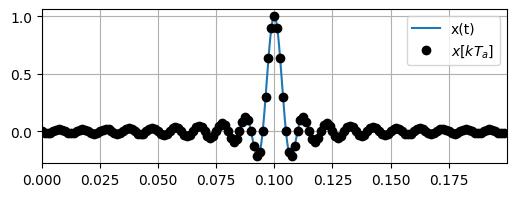
\includegraphics{figuras/nb0_out_1.png}

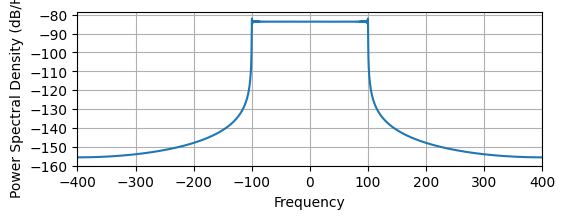
\includegraphics{figuras/nb0_out_2.png}

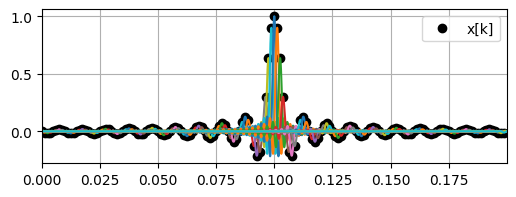
\includegraphics{figuras/nb0_out_3.png}

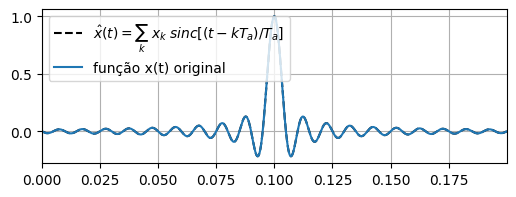
\includegraphics{figuras/nb0_out_4.png}
\end{frame}

\begin{frame}{Exemplo 2: chirp de frequência linear}
\phantomsection\label{exemplo-2-chirp-de-frequuxeancia-linear}
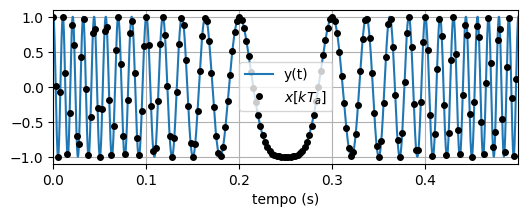
\includegraphics{figuras/nb0_out_5.png}

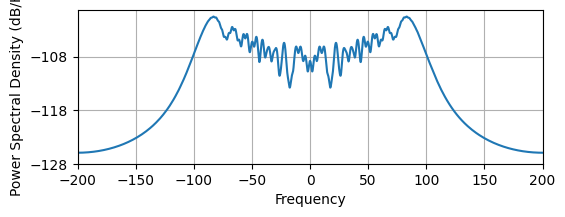
\includegraphics{figuras/nb0_out_6.png}

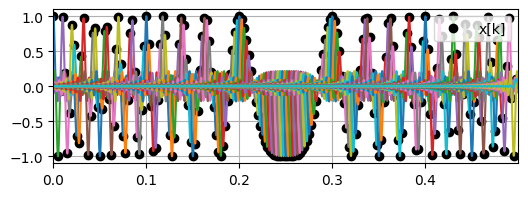
\includegraphics{figuras/nb0_out_7.png}

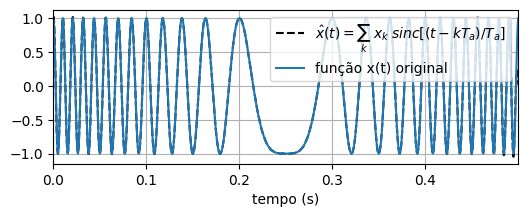
\includegraphics{figuras/nb0_out_8.png}
\end{frame}

\begin{frame}{Formatação de pulso e sinais digitais em banda base}
\phantomsection\label{formatauxe7uxe3o-de-pulso-e-sinais-digitais-em-banda-base}
Partindo de uma sequência de símbolos gerados a partir de um esquema de
modulação digital podemos construir um sinal em banda base na forma de
um trem de pulsos. Seja \(s(t)\) o sinal modulado em banda base
representando a sequência de símbolos \(s_{k}\) formatada com um pulso
\(p(t)\), temos que

\begin{equation} 
s(t) = \sum_{k=-\infty}^{\infty} s_{k} p\left(t-kT_{s}\right)
\end{equation}

com o processo de geração de \(s(t)\) ilustrado na figura a seguir.

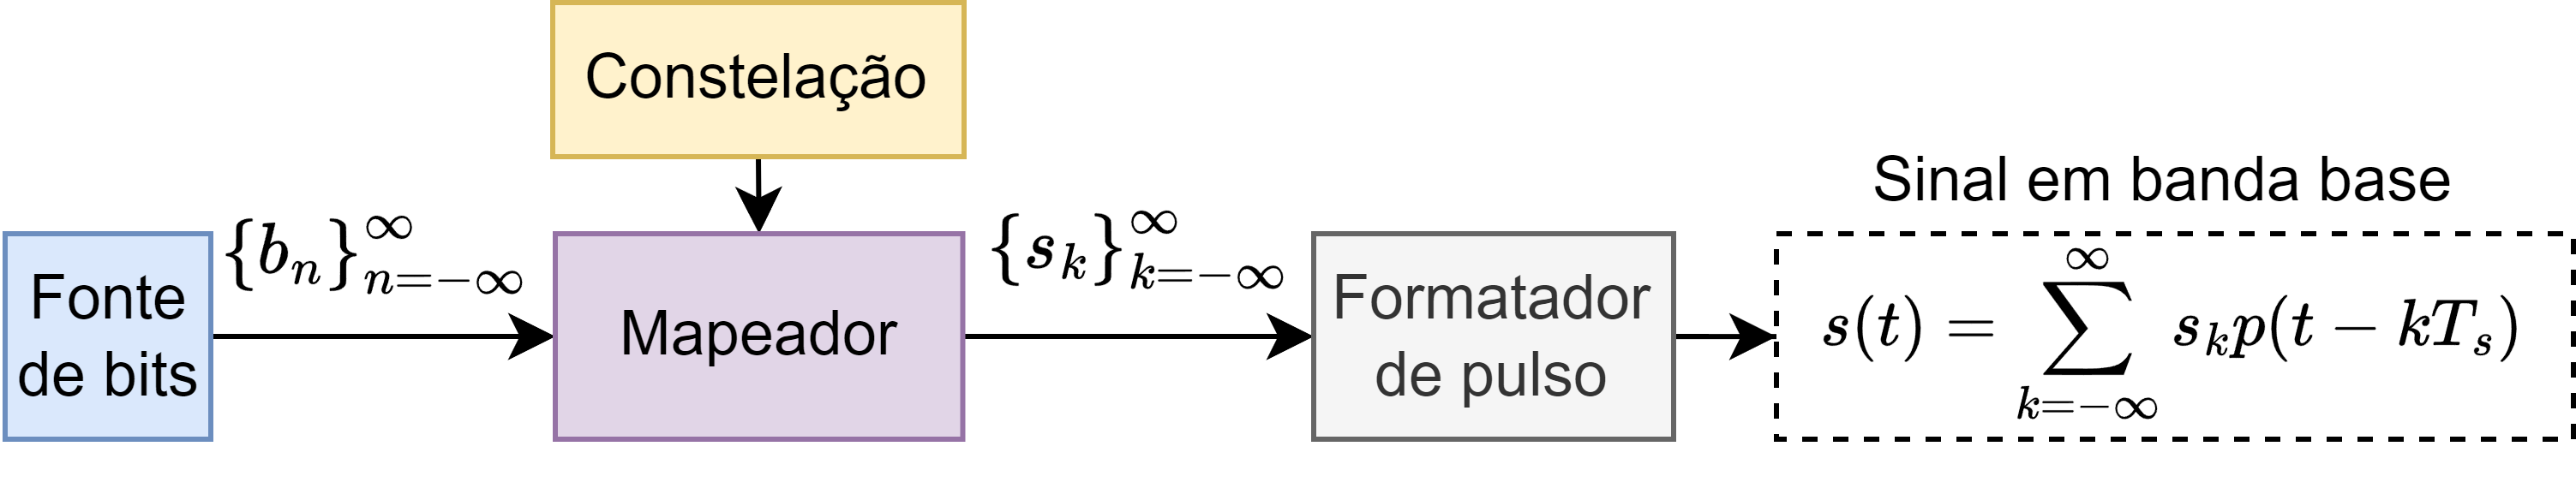
\includegraphics{figuras/Fig1-1.png}

Perceba que \(s(t)\) pode ser gerado a partir de uma convolução entre um
trem de impulsos e o pulso \(p(t)\), i.e.

\begin{align} s(t) &= \left[ \sum_{k=-\infty}^{\infty} s_{k} \delta \left(t-k T_{s}\right)\right] \ast p(t) \nonumber \\ & = \sum_{k=-\infty}^{\infty} s_{k} p\left(t-k T_{s}\right)\end{align}

O sinal \(s_{k}\), por sua vez, poderá ser transmitido diretamente na
banda base ou utilizado na modulação de uma onda portadora.

\begin{align} 
E(t)&=\operatorname{Re}\left[s(t) \exp \left(j \omega_c t\right)\right]\nonumber\\
&= \operatorname{Re}\left[\sum_{k=-\infty}^{\infty} s_{k} p\left(t-kT_{s}\right)\exp \left(j \omega_c t\right)\right]\nonumber\\
&= \left[\sum_{k=-\infty}^{\infty} \operatorname{Re}[s_{k}] p\left(t-kT_{s}\right)\right]\cos\left(\omega_c t\right) - \left[\sum_{k=-\infty}^{\infty} \operatorname{Im}[s_{k}] p\left(t-kT_{s}\right)\right] \sin\left(\omega_c t\right)
\end{align}

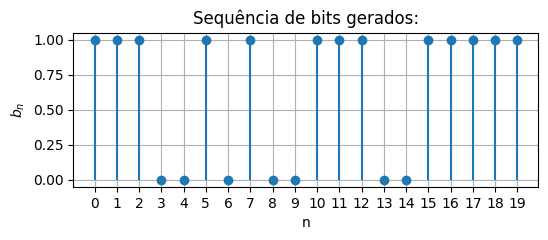
\includegraphics{figuras/nb0_out_9.png}

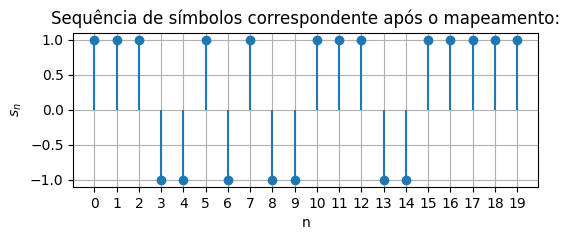
\includegraphics{figuras/nb0_out_10.png}
\end{frame}

\begin{frame}{Pulso retangular ideal}
\phantomsection\label{pulso-retangular-ideal}
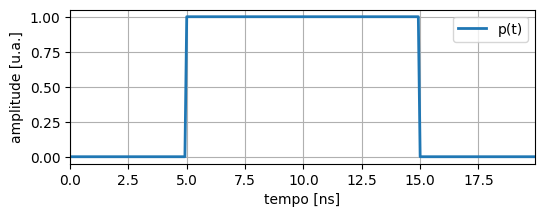
\includegraphics{figuras/nb0_out_11.png}

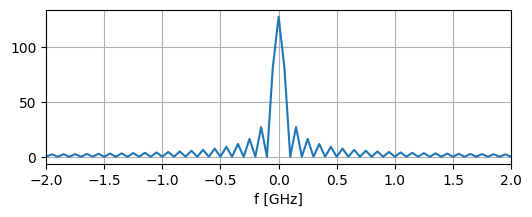
\includegraphics{figuras/nb0_out_12.png}

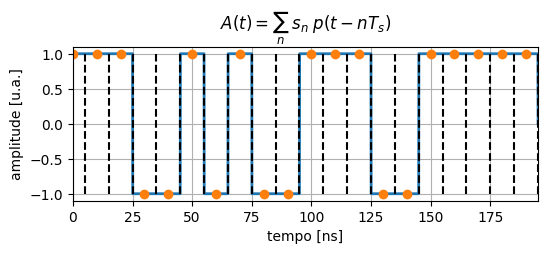
\includegraphics{figuras/nb0_out_13.png}
\end{frame}

\begin{frame}{Pulso NRZ típico}
\phantomsection\label{pulso-nrz-tuxedpico}
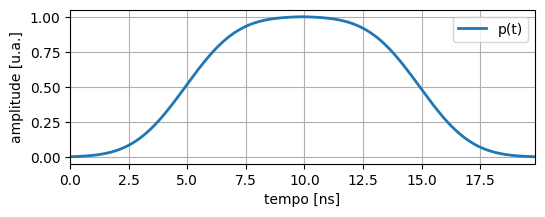
\includegraphics{figuras/nb0_out_14.png}

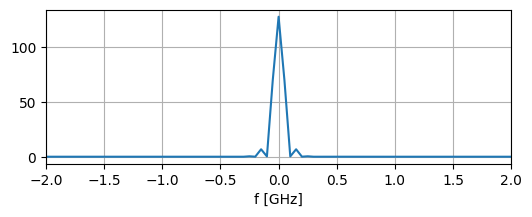
\includegraphics{figuras/nb0_out_15.png}

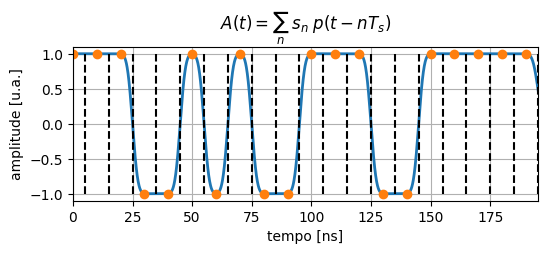
\includegraphics{figuras/nb0_out_16.png}
\end{frame}

\begin{frame}{Pulso cosseno levantado}
\phantomsection\label{pulso-cosseno-levantado}
$$
p(t)=\left\{\begin{array}{ll}
\frac{\pi}{4 T} \operatorname{sinc}\left(\frac{1}{2 \beta}\right), & t=\pm \frac{T}{2 \beta} \\
\frac{1}{T} \operatorname{sinc}\left(\frac{t}{T}\right) \frac{\cos \left(\frac{\pi \beta t}{T}\right)}{1-\left(\frac{2 \beta t}{T}\right)^{2}}, & \text { caso contrário }
\end{array}\right.
$$

$$
P(f)=\left\{\begin{array}{ll}
1, & |f| \leq \frac{1-\beta}{2 T} \\
\frac{1}{2}\left[1+\cos \left(\frac{\pi T}{\beta}\left[|f|-\frac{1-\beta}{2 T}\right]\right)\right], & \frac{1-\beta}{2 T}<|f| \leq \frac{1+\beta}{2 T} \\
0, & \text { caso contrário }
\end{array}\right.
$$

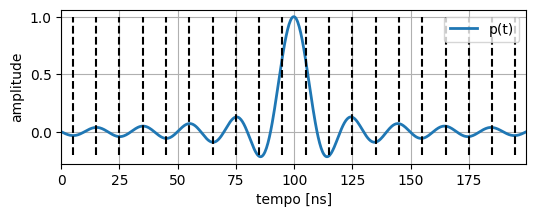
\includegraphics{figuras/nb0_out_17.png}
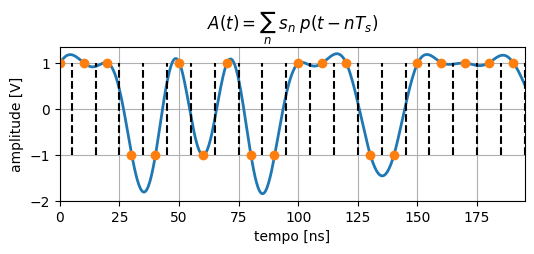
\includegraphics{figuras/nb0_out_18.png}
\end{frame}

\begin{frame}{Densidade espectral de potência de sinais modulados digitalmenente}
\phantomsection\label{densidade-espectral-de-potuxeancia-de-sinais-modulados-digitalmenente}
Considere \(v(t)\) seja um sinal modulado em banda base no domínio do
tempo associado a uma sequência de símbolos \(\{s_n\}\) de um dado
formato de modulação, ou seja

\begin{equation}
v(t)=\sum_{n=-\infty}^{\infty} s_{n} p(t-n T).
\end{equation}

em que \(p(t)\) é o formato do pulso utilizado. O sinal \(v(t)\) pode
ser entendido como uma realização do processo estocástico \(V(t)\) que,
por sua vez, depende da sequência aleatória de símbolos \(\{s_n\}\).
Para cada realização distinta de \(\{s_n\}\) temos uma forma de onda
\(v(t)\) associada.
\end{frame}

\begin{frame}{Valor médio e autocorrelação de \(V(t)\)}
\phantomsection\label{valor-muxe9dio}
\begin{equation}
\begin{aligned}
E[V(t)] &=\sum_{n=-\infty}^{\infty} E\left[s_{n}\right] p(t-n T) \\
&=m_{s} \sum_{n=-\infty}^{\infty} p(t-n T)
\end{aligned}
\end{equation}

Perceba que \(E[V(t)]\) é periódico em \(t\) com período \(T\), que
corresponde ao intervalo de sinalização.
\end{frame}

\begin{frame}{Autocorrelação}
\phantomsection\label{autocorrelauxe7uxe3o}
\begin{equation}
R_{V}(t+\tau, t)=E\left[V^{*}(t) V(t+\tau)\right]=\sum_{n=-\infty}^{\infty} \sum_{m=-\infty}^{\infty} E\left[s_{n}^{*} s_{m}\right] p(t-nT) p(t+\tau-mT)
\end{equation}

Considerando que \(\{s_n\}\) seja uma sequência de símbolos de
informação estacionária no sentido amplo, sua autocorrelação \(R_{s}\) é
definida como

\begin{equation}
\begin{aligned}
R_{s}(n,n+m)&=E\left[s_{n}^{*}s_{n+m}\right]\nonumber\\
        &=R_{s}((n+m)-n)\nonumber\\
        &=R_{s}(m)
\end{aligned}
\end{equation}

Logo, \begin{equation}
R_{V}(t+\tau, t) =\sum_{n=-\infty}^{\infty} \sum_{m=-\infty}^{\infty} R_{s}(m-n) p(t-nT) p(t+\tau-mT).
\end{equation}

Podemos reescrever os somatórios de uma maneira mais conveniente fazendo
a mudança de variáveis \(m'= m-n\), de forma que

\begin{equation}
\begin{aligned}
R_{V}(t+\tau, t) &=\sum_{n=-\infty}^{\infty} \sum_{m=-\infty}^{\infty} R_{s}(m-n) p(t-nT) p(t+\tau-mT)\nonumber\\
                 &=\sum_{n=-\infty}^{\infty} \sum_{m'=-\infty}^{\infty} R_{s}(m') p(t-nT) p(t+\tau-(m'+n)T)\nonumber\\
                 &=\sum_{m'=-\infty}^{\infty} R_{s}(m') \sum_{n=-\infty}^{\infty} p(t-nT) p(t+\tau -nT -m'T)
\end{aligned}
\end{equation}

ou seja, apenas renomeando o índice do somatório, temos

\begin{equation}
R_{V}(t+\tau, t) =\sum_{m=-\infty}^{\infty} R_{s}(m) \sum_{n=-\infty}^{\infty} p(t-nT) p(t+\tau -nT -mT)
\end{equation}

Perceba que também a autocorrelação \(R_{V}(t+\tau, t)\) é periódica em
\(t\) com período \(T\), o que caracteriza \(V(t)\) como um
\emph{processo cicloestacionário}. Desse modo, podemos caracterizar
\(V(t)\) pela sua função de autocorrelação média
\(\bar{R}_{V}(t+\tau, t)\) definida por

\begin{equation}
\begin{aligned}
\bar{R}_{V}(\tau) &=\frac{1}{T} \int_{-T / 2}^{T / 2} R_{V}(t+\tau, t) d t \\
&=\sum_{m=-\infty}^{\infty} R_{s}(m) \sum_{n=-\infty}^{\infty} \frac{1}{T} \int_{-T / 2}^{T / 2} p(t-n T) p(t+\tau-n T-m T) d t \\
&=\sum_{m=-\infty}^{\infty} R_{s}(m) \sum_{n=-\infty}^{\infty} \frac{1}{T} \int_{n T-T / 2}^{n T+T / 2} p(t) p(t+\tau-m T) d t \\
&=\frac{1}{T} \sum_{m=-\infty}^{\infty} R_{s}(m) \int_{-\infty}^{\infty} p(t) p(t+\tau-m T) d t.
\end{aligned}
\end{equation}

A integral \(\int_{-\infty}^{\infty} p(t) p(t+\tau-m T) dt\) é
interpretada como a autocorrelação temporal \(R_{p}(\tau)\) do pulso
\(p(t)\), ou seja

\begin{equation}
R_{p}(\tau)=\int_{-\infty}^{\infty} p(t) p(t+\tau) dt.
\end{equation}

Assim, temos

\begin{equation}
\bar{R}_{V}(\tau)=\frac{1}{T} \sum_{m=-\infty}^{\infty} R_{s}(m) R_{p}(\tau-m T).
\end{equation}
\end{frame}


\begin{frame}{Densidade espectral de potência \(\mathcal{S}_{V}(f)\)}
\phantomsection\label{densidade-espectral-de-potuxeancia-mathcals_vf}
Uma vez estabelecida \(\bar{R}_{V}(\tau)\), podemos utilizar o teorema
de Wiener-Khinchin {[}2{]} para determinar a densidade espectral de
potência \(\mathcal{S}_{V}(f)\) associada a \(V(t)\). O teorema
estabelece que \(\mathcal{S}_{V}(f)\) e \(\bar{R}_{V}(\tau)\) são
relacionadas por meio da transformada de Fourier, ou seja

\begin{equation}
\begin{aligned}
\mathcal{S}_{V}(f) &=\int_{-\infty}^{\infty} \bar{R}_{V}(\tau) e^{-j 2 \pi f \tau} d \tau \\
&=\frac{1}{T} \sum_{m=-\infty}^{\infty} R_{s}(m) \int_{-\infty}^{\infty} R_{p}(\tau-m T) e^{-j 2 \pi f \tau} d \tau \\
&=\frac{1}{T} \sum_{m=-\infty}^{\infty} R_{s}(m) e^{j 2 \pi f m T}\int_{-\infty}^{\infty} R_{p}(\tau) e^{-j 2 \pi f \tau} d \tau \\
&=\frac{1}{T} \sum_{m=-\infty}^{\infty} R_{s}(m) e^{-j 2 \pi f m T}\int_{-\infty}^{\infty} \left[\int_{-\infty}^{\infty} p(t) p(t+\tau) d t\right] e^{-j 2 \pi f \tau} d \tau \\
&=\frac{1}{T} \sum_{m=-\infty}^{\infty} R_{s}(m) e^{-j 2 \pi f m T}\int_{-\infty}^{\infty}p(t) e^{j 2 \pi f t}dt\int_{-\infty}^{\infty}p(\tau)e^{-j 2 \pi f \tau} d \tau \\
&=\frac{1}{T} \mathcal{S}_{s}(f)P^*(f)P(f) \\
&=\frac{1}{T} \mathcal{S}_{s}(f)\left|P(f)\right|^{2}.
\end{aligned}
\end{equation}

Portanto,

\begin{equation}
\mathcal{S}_{V}(f) = \frac{1}{T} \mathcal{S}_{s}(f)\left|P(f)\right|^{2},
\end{equation}

em que \(\mathcal{S}_{s}(f)\) é dada por \begin{equation}
\mathcal{S}_{s}(f)=\sum_{m=-\infty}^{\infty} R_{s}(m) e^{-j 2 \pi f m T}.
\end{equation}

Em resumo, a densidade espectral de potência de \(\mathcal{S}_{V}(f)\)
depende de dois parâmetros:

\begin{enumerate}
\tightlist
\item
  Do espectro de potência associado à transformada de Fourier \(P(f)\)
  do pulso \(p(t)\).
\item
  Das caraterísticas espectrais \(\mathcal{S}_{s}(f)\) da sequência de
  símbolos de informação \(\{s_n\}\).
\end{enumerate}

No caso particular, que engloba a maioria das situações práticas, os
símbolos em \(\{s_n\}\) são mutuamente descorrelacionados, de forma que

\begin{equation}
R_{s}(m) = \begin{cases}\sigma_{s}^{2}+m_{s}^{2}, & m=0 \\ m_{s}^{2}, & m \neq 0\end{cases}
\end{equation}

em que \(\sigma_{s}^{2}+m_{s}^{2}=E[s^2]\) é a energia média dos
símbolos da constelação.

ou seja,

\begin{equation}
\mathcal{S}_{s}(f)=\sigma_{s}^{2}+m_{s}^{2} \sum_{m=-\infty}^{\infty} e^{-j 2 \pi f m T}
\end{equation}

Utilizando a relação entre um trem trem de impulsos no domínio da
frequência e sua representação em termos da série de Fourier, temos que

\begin{equation}
\sum_{n=-\infty}^{\infty} e^{-j 2 \pi f mT}=\frac{1}{T} \sum_{m=-\infty}^{\infty} \delta\left(f-\frac{m}{T}\right).
\end{equation}

Assim, podemos reescrever

\begin{equation}
\mathcal{S}_{s}(f)=\sigma_{s}^{2}+\frac{m_{s}^{2}}{T} \sum_{m=-\infty}^{\infty} \delta\left(f-\frac{m}{T}\right).
\end{equation}

Finalmente, \(\mathcal{S}_{V}(f)\) será dada por

\begin{equation}
\mathcal{S}_{V}(f)=\frac{\sigma_{s}^{2}}{T}\left|P(f)\right|^{2}+\frac{m_{s}^{2}}{T^{2}} \sum_{m=-\infty}^{\infty}\left|P\left(\frac{m}{T}\right)\right|^{2} \delta\left(f-\frac{m}{T}\right).
\end{equation}

De maneira geral, as constelações dos formatos de modulação ASK, PSK,
QAM são definidas de tal forma que \(m_{s}=0\), bastando apenas que os
símbolos sejam posicionados de forma simétrica no plano complexo. Nesse
caso, temos

\begin{equation}
\mathcal{S}_{V}(f)=\frac{\sigma_{s}^{2}}{T}\left|P(f)\right|^{2}
\end{equation}

ou seja, o formato de \(\mathcal{S}_{V}(f)\) depende apenas do tipo de
pulso \(p(t)\) escolhido.

Para mais detalhes, ver capítulo 8 de {[}2{]}.
\end{frame}

\begin{frame}{Exemplos de densidade espectral de potência de sinais
modulados}
\phantomsection\label{exemplos-de-densidade-espectral-de-potuxeancia-de-sinais-modulados}
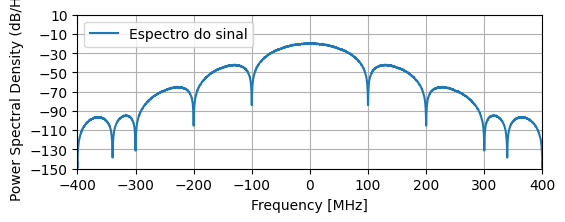
\includegraphics{figuras/nb0_out_19.png}
\end{frame}

\begin{frame}{Diagramas de olho}
\phantomsection\label{diagramas-de-olho}
Um diagrama de olho é uma representação gráfica por meio da qual pode-se
aferir a qualidade de um sinal num sistema de comunicação digital. Ele é
usado para visualizar a forma de onda do sinal e a sua integridade,
permitindo a avaliação de métricas de qualidade do sinal e a
identificação de possíveis problemas, como interferências ou distorções.
Um exemplo de um diagrama de olho para um sinal binário NRZ está
ilustrado na figura abaixo.

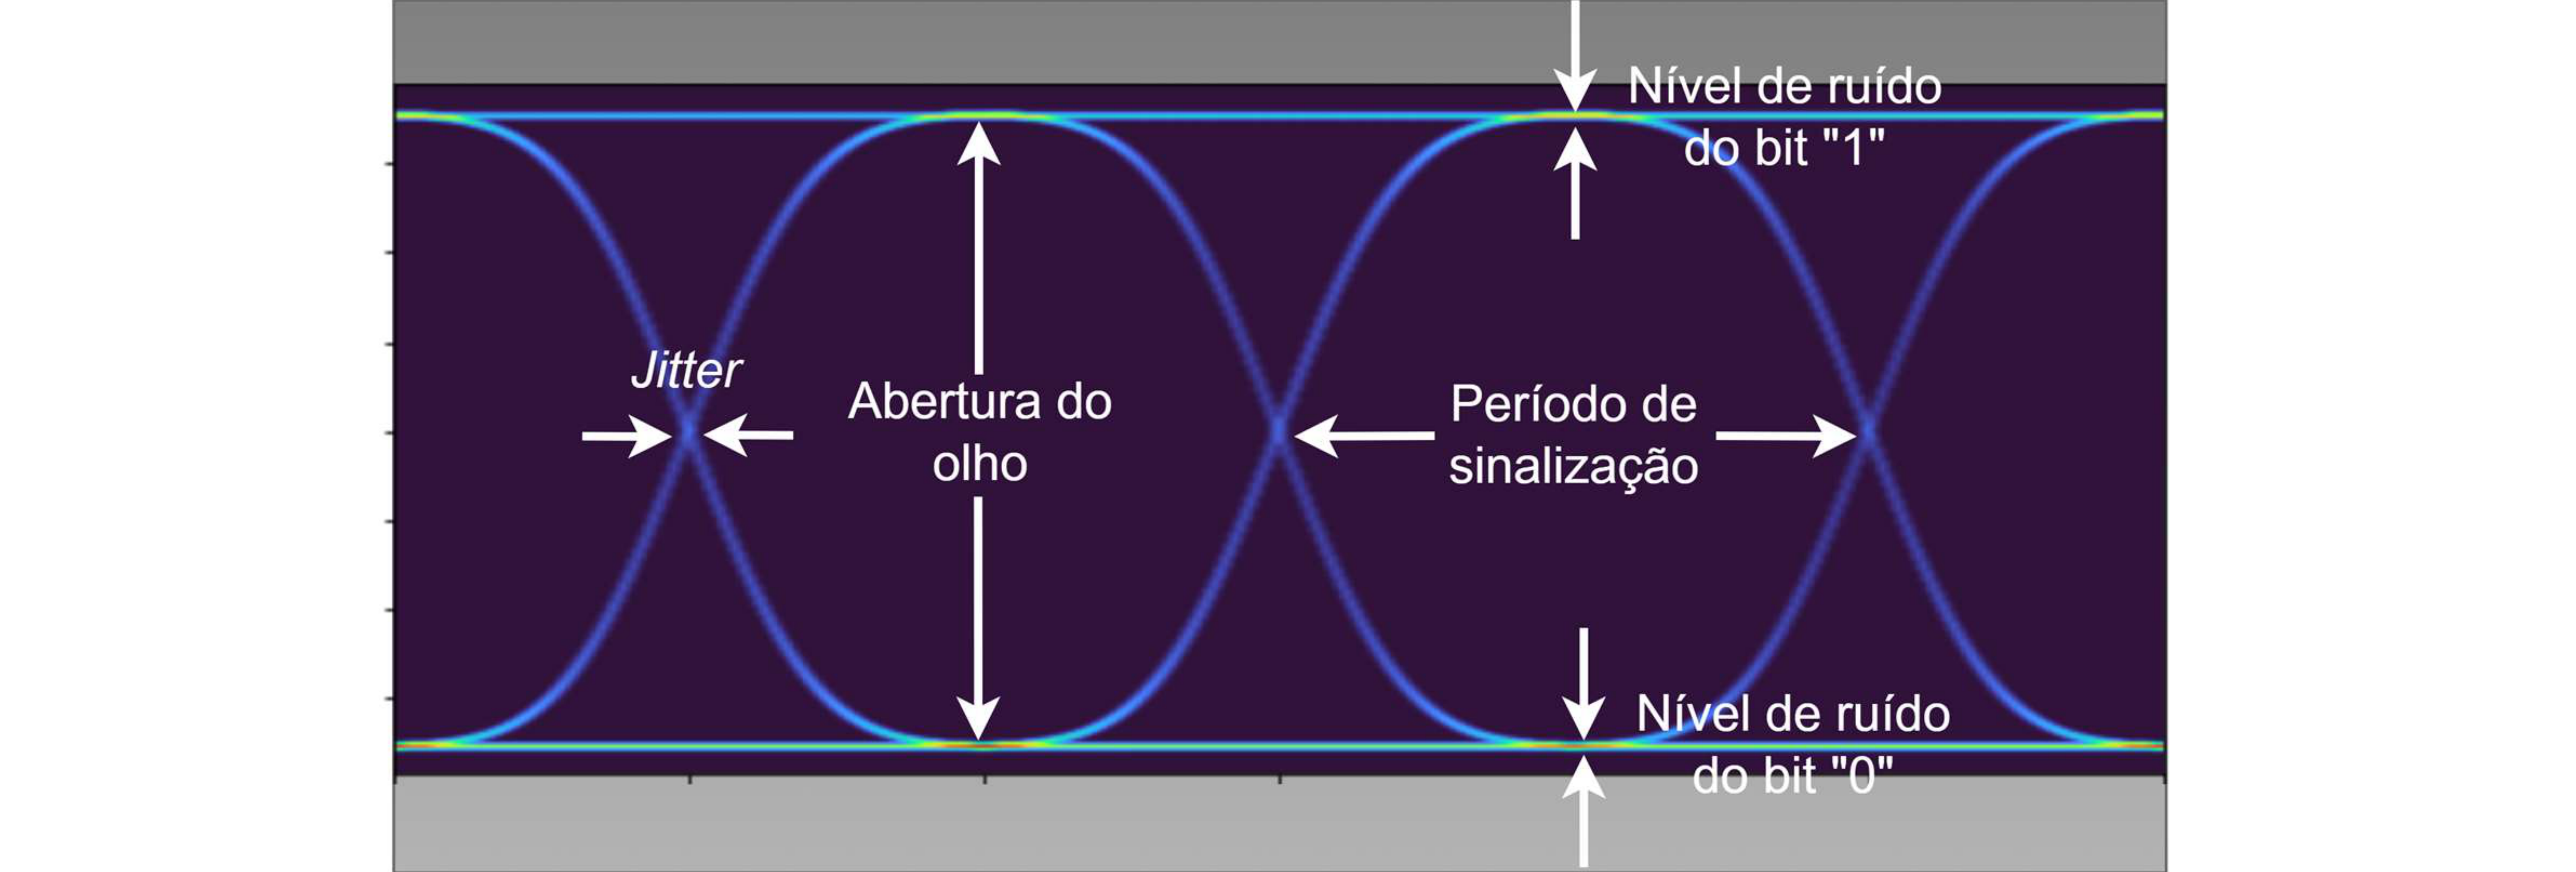
\includegraphics{figuras/Fig2.png}

O diagrama de olho é composto por um conjunto de curvas que representam
a variação do sinal ao longo do tempo. Cada curva é gerada pela
sobreposição de várias amostras do sinal, permitindo que sejam
identificadas as variações que ocorrem durante a transmissão. O ponto
central do diagrama de olho representa a posição média do sinal,
enquanto as curvas que se estendem para cima e para baixo representam as
variações que ocorrem durante a transmissão.
\end{frame}

\begin{frame}{Modulação M-PAM}
\phantomsection\label{diagramas-de-constelauxe7uxe3o-1}
\end{frame}

\begin{frame}{Mapeando bits para símbolos}
\phantomsection\label{mapeando-bits-para-suxedmbolos}
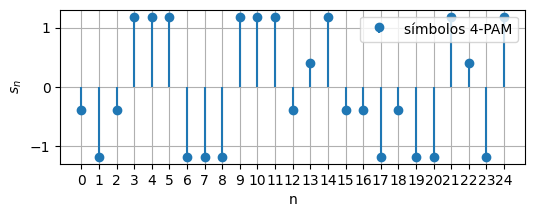
\includegraphics{figuras/nb0_out_20.png}

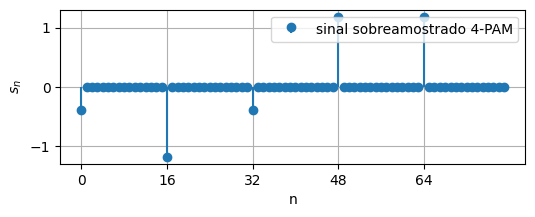
\includegraphics{figuras/nb0_out_21.png}

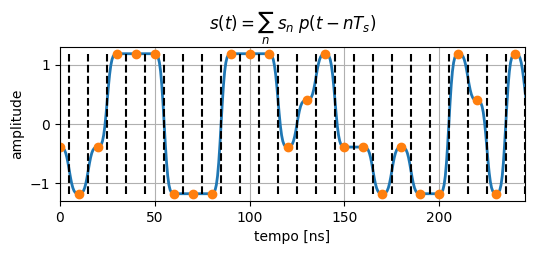
\includegraphics{figuras/nb0_out_22.png}

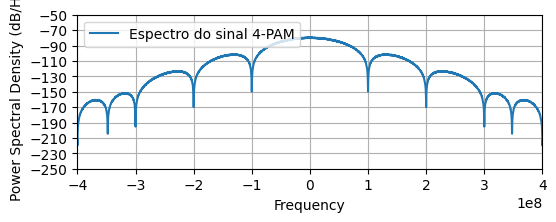
\includegraphics{figuras/nb0_out_23.png}
\end{frame}

\begin{frame}{Diagramas de olho}
\phantomsection\label{diagramas-de-olho-1}
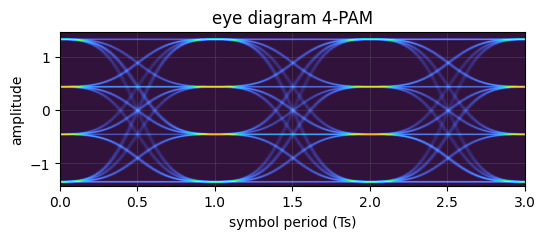
\includegraphics{figuras/nb0_out_24.png}
\end{frame}

\begin{frame}{Modulação M-QAM}
\phantomsection\label{modulauxe7uxe3o-m-qam}
\phantomsection\label{diagramas-de-constelauxe7uxe3o-2}
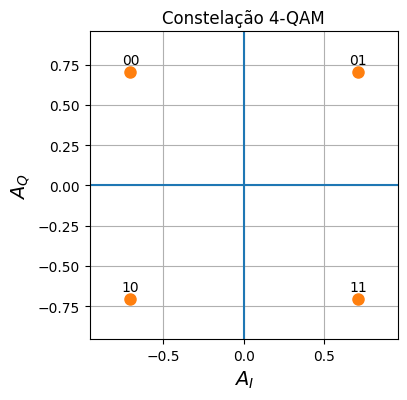
\includegraphics{figuras/nb0_out_25.png}
\end{frame}

\begin{frame}{Mapeando bits para símbolos}
\phantomsection\label{mapeando-bits-para-suxedmbolos-1}
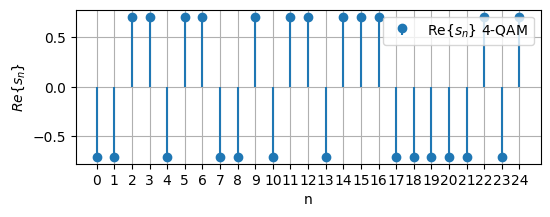
\includegraphics{figuras/nb0_out_26.png}

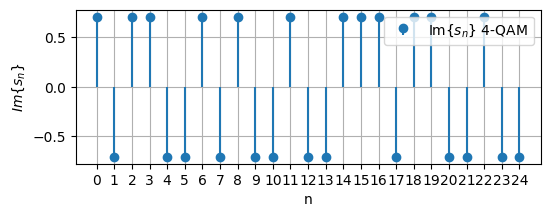
\includegraphics{figuras/nb0_out_27.png}

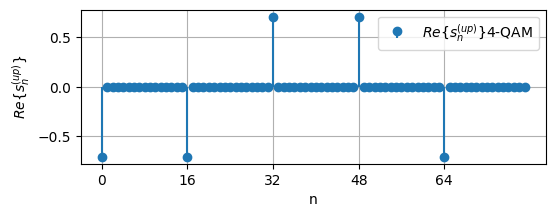
\includegraphics{figuras/nb0_out_28.png}

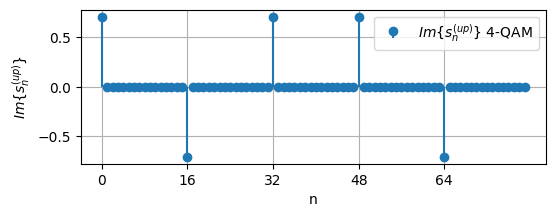
\includegraphics{figuras/nb0_out_29.png}

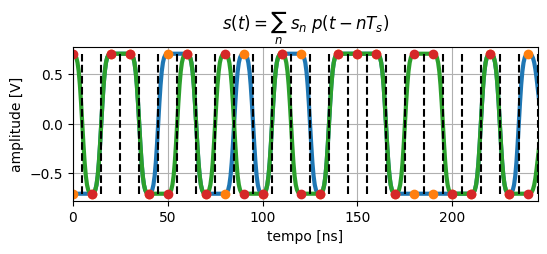
\includegraphics{figuras/nb0_out_30.png}
\end{frame}

\begin{frame}{Espectro do sinal modulado}
\phantomsection\label{espectro-do-sinal-modulado}
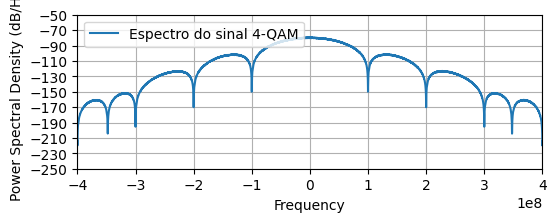
\includegraphics{figuras/nb0_out_31.png}
\end{frame}

\begin{frame}{Diagramas de olho}
\phantomsection\label{diagramas-de-olho-2}
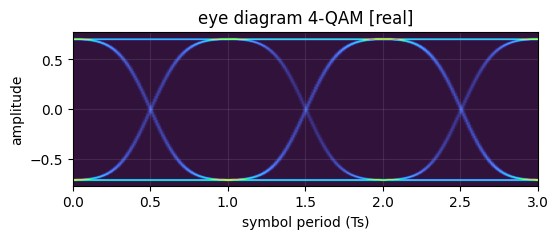
\includegraphics{figuras/nb0_out_32.png}

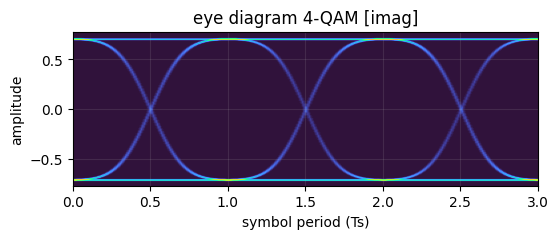
\includegraphics{figuras/nb0_out_33.png}

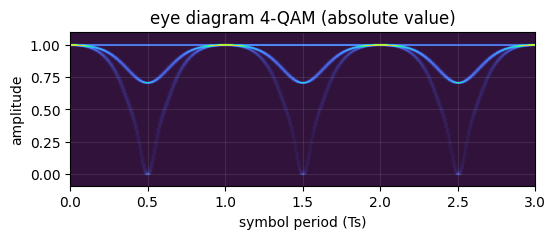
\includegraphics{figuras/nb0_out_34.png}
\end{frame}


\begin{frame}{Modulação M-PSK}
\phantomsection\label{diagramas-de-constelauxe7uxe3o-3}
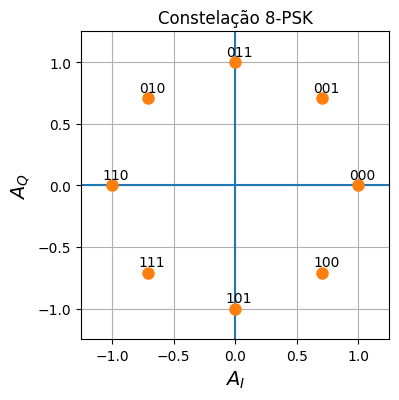
\includegraphics{figuras/nb0_out_35.png}
\end{frame}

\begin{frame}{Mapeando bits para símbolos}
\phantomsection\label{mapeando-bits-para-suxedmbolos-2}
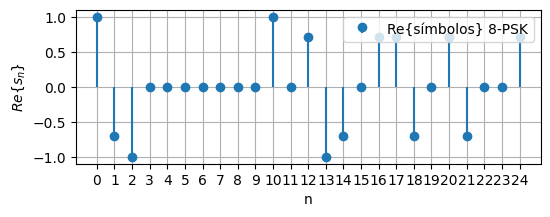
\includegraphics{figuras/nb0_out_36.png}

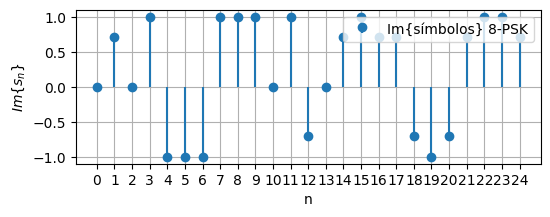
\includegraphics{figuras/nb0_out_37.png}

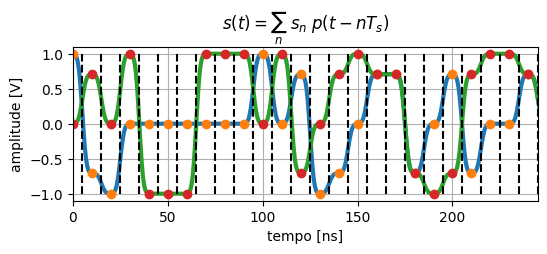
\includegraphics{figuras/nb0_out_38.png}
\end{frame}

\begin{frame}{Espectro do sinal modulado}
\phantomsection\label{espectro-do-sinal-modulado-1}
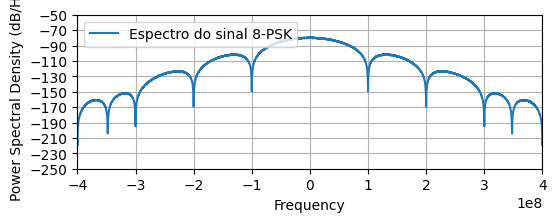
\includegraphics{figuras/nb0_out_39.png}
\end{frame}

\begin{frame}{Diagramas de olho}
\phantomsection\label{diagramas-de-olho-3}
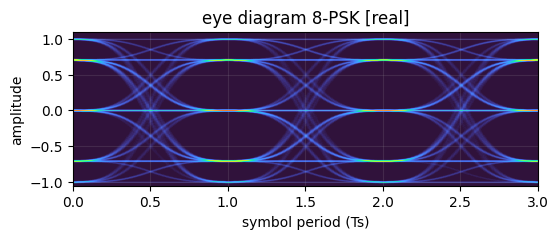
\includegraphics{figuras/nb0_out_40.png}

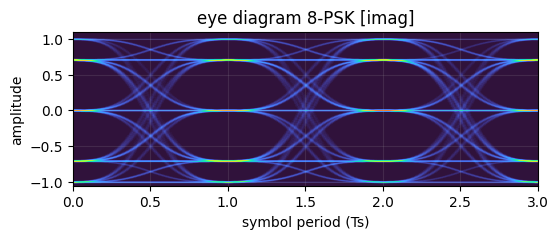
\includegraphics{figuras/nb0_out_41.png}

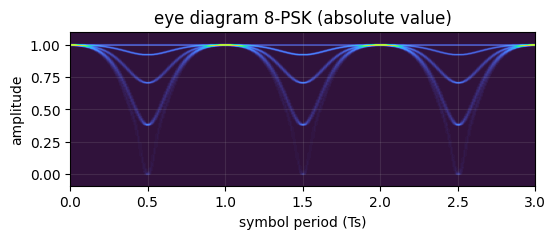
\includegraphics{figuras/nb0_out_42.png}
\end{frame}

\begin{frame}{Referências}
\phantomsection\label{referuxeancias}
{[}1{]} J. G. Proakis, M. Salehi, Communication Systems Engineering, 2nd
Edition, Pearson, 2002.
\end{frame}

\end{document}
